\documentclass[11pt]{extreport}

\usepackage[top=2.5cm,bottom=2.5cm,left=3.5cm,right=2.5cm,a4paper]{geometry} % Page margins

% Packages for formatting and functionality
\usepackage{csvsimple}
\usepackage{graphicx} % For including images
\usepackage[T1]{fontenc} % Font encoding
\usepackage[utf8]{inputenc} % Input encoding
\usepackage[polish]{babel} % Polish language support
\usepackage{tgtermes} % Times New Roman font
\usepackage{titlesec} % Customizing section titles
\usepackage{tocloft} % Customizing table of contents
\usepackage{setspace} % Line spacing
\usepackage{indentfirst} % Indent first paragraph of sections
\usepackage{ragged2e} % Justify text
\usepackage[format=plain,
            labelfont=it,
            textfont=it,
            labelsep=period,
            justification=centering]{caption}% Image decription

\usepackage{minted} % Code blocks
\usepackage[style=ieee]{biblatex}
\usepackage{csquotes}
\usepackage{afterpage}
\usepackage{amsmath}
\usepackage{hyperref}
\hypersetup{colorlinks,%
citecolor=black,%
filecolor=black,%
linkcolor=black,%
urlcolor=black,%
}


% Path to images
\graphicspath{ {./images/} }

% Customizing figure captions
\makeatletter
\renewcommand{\fnum@figure}{Rys. \thefigure}
\makeatother

% Customizing spacing for chapters, sections, and subsections
\titlespacing*{\chapter}{0pt}{0pt}{6pt}
\titlespacing*{\section}{6pt}{6pt}{6pt}
\titlespacing*{\subsection}{6pt}{6pt}{6pt}

% Customizing table of contents title font
\renewcommand{\cfttoctitlefont}{\fontsize{16}{18}\selectfont\bfseries}

% Settings for paragraph indentation and line spacing
\setlength{\parindent}{0.63cm}
\setstretch{1.25}

% Justify paragraphs
\justifying

% Customizing section font size to 13pt
\titleformat{\section}
  {\normalfont\fontsize{13}{15}\bfseries} % Font size and style
  {\thesection}{1em}{}

% Customizing subsection font size to 12pt
\titleformat{\subsection}
  {\normalfont\fontsize{12}{14}\bfseries} % Font size and style
  {\thesubsection}{1em}{}
  
% Ustawienia bloków kodu 
\setminted{
  frame=single,
  baselinestretch=1
  }


\makeatletter
\renewcommand{\@makechapterhead}[1]{%
  {\parindent \z@ \raggedright 
    \ifnum \c@secnumdepth >\m@ne
      \fontsize{14}{16}\bfseries \thechapter\quad
    \fi
     \fontsize{14}{16} \bfseries #1\par\nobreak
    \vskip 6\p@
  }}
\makeatother

\addbibresource{bibliografia.bib}


\newcommand\blankpage{%
    \null
    \thispagestyle{empty}%
    \addtocounter{page}{-1}%
    \newpage}

\let\tempone\itemize
\let\temptwo\enditemize
\renewenvironment{itemize}{\tempone\addtolength{\itemsep}{-0.4\baselineskip}}{\temptwo}

\begin{document}

% Dla lepszej wydajności można w trakcie pisania zakomentować obydwa include
\begin{titlepage}

% Redu marginile
\newgeometry{left=2cm,right=2cm,bottom=1cm}

\begin{figure}[!htb]
    \centering
    \begin{minipage}{0.2\textwidth}
        
\includegraphics[width=0.7\linewidth]{images/loga/PK_logo.jpg}
    \end{minipage}
    \begin{minipage}{0.5\textwidth}
        \large
        \vspace{0.2cm}
        \fontsize{14pt}{16pt}\selectfont
        \begin{center}
            \textbf{POLITECHNIKA KRAKOWSKA \\ im. T. Kościuszki}
        \end{center}
        \begin{center}
                Wydział Mechaniczny \\
                \textbf{Katedra (uzupełnić)
                }
        \end{center}
    \end{minipage}
    \begin{minipage}{0.2\textwidth}
        
\includegraphics[width=0.7\linewidth]{images/loga/wm_logo.jpg}
    \end{minipage}
\end{figure}

\begin{flushleft}
\fontsize{14pt}{16pt}\selectfont
Kierunek studiów: \\
Specjalność: 
\end{flushleft}

\vspace{1cm}

\begin{center}
\fontsize{14pt}{16pt}\selectfont
STUDIA STACJONARNE/NIESTACJONARNE
\end{center}

\vspace{0.5cm}
\begin{center}
\fontsize{24pt}{26pt}\selectfont
\textbf{PRACA DYPLOMOWA} \\
\end{center}
\begin{center}
\fontsize{12pt}{14pt}\selectfont
INŻYNIERSKA/MAGISTERSKA
\end{center}
\vspace{0.5cm}
\begin{center}
\fontsize{14pt}{16pt}\selectfont
\textbf{Imię i nazwisko}
\end{center}
\vspace{0.5cm}
\begin{center}
\fontsize{14pt}{16pt}\selectfont

Temat pracy dyplomowej w języku polskim \\
\vspace{0.3cm}

Temat pracy dyplomowej w języku angielskim

\end{center}

\vspace{2cm}


\begin{center}
\large Promotor: \\ Tytuł/stopień naukowy \textbf{Imię i nazwisko}
\end{center}

\vspace{1cm}

\begin{center}
\Large Kraków, rok akad. 2025/2026
\end{center}
\end{titlepage}

\shipout\null


\begingroup
\begin{small}
\begin{center}
     \large  \textbf{ OŚWIADCZENIE O SAMODZIELNYM WYKONANIU \\ PRACY DYPLOMOWEJ}
\end{center}

Oświadczam, że przedkładana przeze mnie praca dyplomowa \textbf{magisterska/inżynierska} została napisana przeze mnie samodzielnie. Jednocześnie oświadczam, że ww. praca: 
\begin{enumerate}
\item nie narusza praw autorskich w rozumieniu ustawy z dnia 4 lutego 1994 r. o prawie autorskim i prawach pokrewnych (Dz.U. z 2021 r. poz. 1062) oraz dóbr osobistych chronionych prawem cywilnym, a także nie zawiera danych i informacji, które uzyskałem/am* w sposób niedozwolony,
\item nie była wcześniej podstawą żadnej innej procedury związanej z nadawaniem tytułów zawodowych, stopni lub tytułów naukowych.

\end{enumerate}

Jednocześnie wyrażam zgodę na:


\begin{enumerate}

\item poddanie mojej pracy kontroli za pomocą systemu Antyplagiat oraz na umieszczenie tekstu pracy w bazie danych uczelni, w celu ochrony go przed nieuprawnionym wykorzystaniem. Oświadczam, że zostałem/am* poinformowany/a* i wyrażam zgodę, by system Antyplagiat porównywał tekst mojej pracy z tekstem innych prac znajdujących się w bazie danych uczelni, z tekstami dostępnymi w zasobach światowego Internetu oraz z bazą porównawczą systemu Antyplagiat,
\item to, aby moja praca pozostała w bazie danych uczelni przez okres wynikający z przepisów prawa. Oświadczam, że zostałem poinformowany i wyrażam zgodę, że tekst mojej pracy stanie się elementem porównawczej bazy danych uczelni, która będzie wykorzystywana, w tym także udostępniana innym podmiotom, na zasadach określonych przez uczelnię, w celu dokonywania kontroli antyplagiatowej prac dyplomowych/doktorskich, a także innych tekstów, które powstaną w przyszłości.



\begin{flushright}
……………………………… \\
podpis
\end{flushright}


\item Wyrażam zgodę na udostępnianie mojej pracy dyplomowej w Akademickim Systemie Archiwizacji Prac na PK do celów naukowo-badawczych z poszanowaniem przepisów ustawy o prawie autorskim i prawach pokrewnych (Dz.U. z 2021 r. poz. 1062)..

 
\begin{flushright}
TAK/NIE* \\
………………………………\\
podpis
\end{flushright}

\end{enumerate}
\textit{Jednocześnie przyjmuję do wiadomości, że w przypadku stwierdzenia popełnienia przeze mnie czynu polegającego na przypisaniu sobie autorstwa istotnego fragmentu lub innych elementów cudzej pracy, lub ustalenia naukowego, Rektor PK stwierdzi nieważność postępowania w sprawie nadania mi tytułu zawodowego (art. 77 ust. 5 ustawy z dnia 18 lipca 2018 r. Prawo o szkolnictwie wyższym i nauce, (Dz.U. z 2021 r., poz. 478, z późn. zm.)).}

\begin{flushright}
……………………………… \\
podpis
\end{flushright}
\end{small}

\endgroup

\afterpage{\blankpage}
\tableofcontents  %Spis treści

\begingroup
\titleformat{\chapter}[hang]
  {\normalfont\fontsize{16}{20}\bfseries}
  {\thechapter.}{1em}{}

\addcontentsline{toc}{chapter}{Wykaz oznaczeń}      % Opcjonalny wykaz oznaczeń
\chapter*{Wykaz oznaczeń}                           
\endgroup

\chapter{Cel i zakres pracy}              %rozdział

(Styl Standardowy, Times New Roman 11 lub Arial 11, odstęp między liniami tekstu 1.25 wiersza, wcięcie pierwszego wiersza: 0,6). W rozdziale „Cel i zakres pracy” należy przedstawić jasno, co jest przedmiotem pracy. Wyjaśnić cel oraz podać czynności, które zostały wykonane, aby ten cel został osiągnięty. W rozdziale tym można opisać z czego praca będzie się składać, np.: 
Niniejsza praca dyplomowa składać się będzie z dwóch głównych części. Pierwsza z nich poświęcona zostanie omówieniu zagadnień teoretycznych, związanych z wykorzystaniem energii słonecznej, a w szczególności … Druga część tej pracy związana będzie bezpośrednio z wykonywanym projektem…
Jeżeli zostało użyte oprogramowanie przy realizacji pracy należy to oprogramowanie wymienić. Rozdział „Cel i zakres pracy” powinien zając maksymalnie jedną stronę. 

\chapter{Wstęp} 

Tekst pracy należy napisać czcionką Time New Roman 11 lub Arial 11, odstęp 1.25 wiersza, wcięcie pierwszego wiersza: 0,63 (Styl Standardowy). Do całości pracy zastosować wyjustowanie akapitów, lewy margines ma wynosić 3.5 cm natomiast pozostałe marginesy 2.5 cm. Przy drukowaniu pracy należy uwzględni fakt, że jeden z egzemplarzy ma zostać wydrukowany dwustronnie i oprawiony w miękkie oprawki (marginesy lustrzane). Rozdziały główne pracy powinny być umieszczone na następnej (nowej) stronie.

\chapter{Układ graficzny pracy}

Przy pisaniu pracy obowiązuje styl bezosobowy tak jak pokazują to poniższe przykłady: 
Wpływ zachmurzenia na gęstość strumienia promieniowania słonecznego przedstawiono na rysunku 3.1.  – \textbf{poprawnie}
Wpływ zachmurzenia na gęstość strumienia promieniowania słonecznego przedstawia rysunek 3.1.  – \textbf{poprawnie}
Wpływ zachmurzenia na gęstość strumienia promieniowania słonecznego przedstawiłem na rysunku 3.1. – \textbf{niepoprawnie}

\begin{figure}[ht]
    \centering
    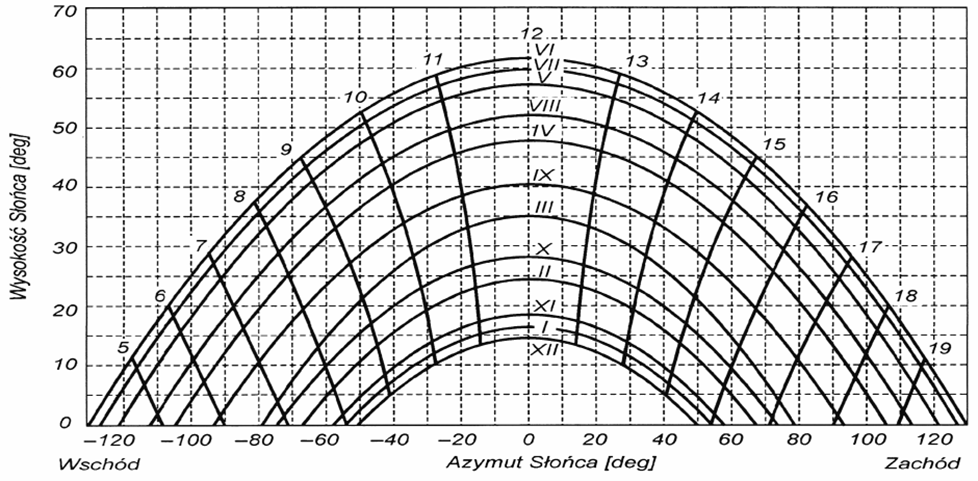
\includegraphics[width=0.80\linewidth]{images/Obraz2.png}
    \caption{Wysokość i azymut Słońca dla 52°N \cite{dirac} }
    \label{fig:Obraz2}
\end{figure}
Styl RYS, Times New Roman 11, kursywa, odstęp pomiędzy wierszami pojedynczy. W podpisach rysunków nie dajemy kropki na końcu

\section{Wzory} %podrozdział (h2)

Jeżeli występują w tekście wzory należy je numerować oraz podać opis wielkości w nich występujących. Wzory należy wyśrodkowywać a numerowanie worów wyrównywać do prawej krawędzi tak jak przedstawia to poniższy przykład. Zmienne we wzorach powinny być napisane kursywą. Wzór jest częścią zadania, obowiązują w związku z tym zasady interpunkcji.   

\subsection{Natężenia promieniowania } %podrozdział (h3)

Przykład:
Chwilowa wartość natężenia promieniowania jest parametrem, który wylicza się z zależności:

\begin{equation}
  G'min = U\underset{L}{}*\frac{\Delta T}{\eta\underset{opt}{} } \tag{3.1}\label{eq:3.1} 
\end{equation}

gdzie: \\
$\eta\underset{opt}{}$ - sprawność optyczna kolektora, \\
$U\underset{L}{}$- współczynnik całkowitych strat kolektora, [W/m2K],\\
$\Delta T$ - różnica temperatur pomiędzy czynnikiem solarnym a otoczeniem, [K].\\

\section{Rysunki, tabele i bloki kodu}

Rysunki oraz tabele (tylko dobrej jakości, min. 300dpi) występujące w tekście należy wyśrodkowywać. Każdy rysunek oraz tabela musi zawierać numer oraz podpis. Podpis umieszcza się pod rysunkiem oraz nad tabelą, tak jak to przedstawiają poniższe przykłady. Odstęp pomiędzy tekstem a rysunkiem wynosi jedną linię. \textbf{Uwaga!} Nie można wstawiać do pracy rysunków oraz tabel bez ich opisu/komentarza w tekście. Rysunek lub tabela pozbawione komentarzy w tekście są bezwartościowe i obniżają jakość pracy. 
Przykład: Wysokość i azymut Słońca we wszystkich porach roku przedstawia rysunek 2.1. Gęstość strumienia promieniowania zależy od zachmurzenia co ilustruje rys.2.2. \\

\begin{figure}[ht]
    \centering
    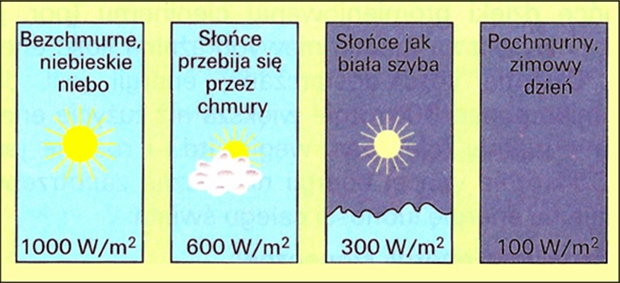
\includegraphics[width=0.75\linewidth]{images/Obraz3.png}
    \caption{Wpływ zachmurzenia na gęstość strumienia promieniowania }
    \label{fig:Obraz3}
\end{figure}

Wstawiane do pracy rysunki, schematy, wykresy, zdjęcia są traktowane jak rysunki i nie rozróżnia się ich w podpisach. Pomimo tego, że wstawiany jest wykres podpisywany jest on jako kolejny rysunek. Rysunki umieszcza się w pracy przez wstawienie z pliku *.jpg.
Numeracje rysunków, tabel oraz wzorów przeprowadza się w obrębie głównych rozdziałów. Wyniki obliczeń dla poszczególnych miesięcy przedstawia tabela 2.1.

\subsection{Tabela manualna}

\begin{table}[ht]
\centering			          %justowanie całej tabeli na środku strony
\caption{Przykładowa tabela}  %opis tabeli
\label{tab:przyklad}		  %etykieta, przyda się do odwołań
\begin{tabular}{|c|c|c|}      %justowanie c-enter, l-eft, r-ight
\hline					      %pozioma linia
Dane 1 & Dane 2 & Dane 3 \\
\hline                                 % linia pozioma
Komórka 1 & Komórka 2 & Komórka 3 \\  % & oddziela kolumny
\hline
Komórka 4 & Komórka 5 & Komórka 6 \\  % \\ zamyka kolumnę
\hline
\end{tabular}
\end{table}

\subsection{Tabela z pliku csv}
To Do

\subsection{Blok kodem programu }
Można również bezpośrednio z pliku % \inputminted{python}{filename.py}
\begin{minted}{python}

def f(x):
    return 1/(1 + x**2)

# Implementing trapezoidal method
def trapezoidal(x0,xn,n):
    # calculating step size
    h = (xn - x0) / n
    
    # Finding sum 
    integration = f(x0) + f(xn)
    
    for i in range(1,n):
        k = x0 + i*h
        integration = integration + 2 * f(k)
    
    # Finding final integration value
    integration = integration * h/2
    
    return integration
\end{minted}

\section{Cytowany tekst }

W przypadku cytowania fragmentów tekstów, tabel, rysunków lub wzorów z literatury należy zaznaczyć autora tego cytowania w tekście pracy.

\textbf{Sposób pierwszy:} Cytowanie poprzez umieszczenie odpowiedniego numeru w nawiasie kwadratowym. Powołanie na literaturę umieszcza się po cytowanym fragmencie teksu przed kropką np.: Na skutek procesów zachodzących w atmosferze, do powierzchni Ziemi dociera jedynie 39-45\% promieniowania pozaatmosferycznego w skali roku [10].  - \textbf{poprawnie}    
Na skutek procesów zachodzących w atmosferze, do powierzchni Ziemi dociera jedynie 39-45\% promieniowania pozaatmosferycznego w skali roku. [10]  - \textbf{niepoprawnie }

\textbf{Sposób drugi:} Cytowanie poprzez powołanie się na autorów cytowanej pracy oraz roku publikacji pracy np.: Nowak i Kowalski (2009) w swojej pracy prezentują … 
Jeżeli autorami pracy są więcej niż dwie osoby należy użyć w cytowaniu tylko nazwiska pierwszego autora np.: Nowak i inni (2010) w swojej pracy prezentują …
Jeżeli ci sami autorzy (lub autor) w jednym roku wydali kilka publikacji, które są w pracy cytowane należy po roku cytowanej publikacji dodać jeszcze literę zgodnie z kolejnością umieszczenia publikacji w wykazie literatury np.: Nowak (2011a) oraz Nowak (2011c) w swoich pracach przedstawia …

\chapter{Wnioski}

We wnioskach należy w przejrzysty sposób podsumować pracę, napisać czy założony cel pracy został osiągnięty i w jakim stopniu. Jeżeli praca ma charakter projektu, autor powinien podać zalecenia projektowe wynikające z przeprowadzonych obliczeń/analiz. Jeżeli z pracy wynikają wnioski przyszłościowe należy je wymienić. Należy użyć stylu, rozmiaru czcionki i odstępu takich jak w całej pracy.


\printbibliography[title={Literatura}]

\begingroup
\titleformat{\chapter}[hang]
  {\normalfont\fontsize{16}{20}\bfseries\centering}
  {\thechapter.}{1em}{}

\addcontentsline{toc}{chapter}{Summary}      % Opcjonalny wykaz oznaczeń
\chapter*{Summary}                           
\endgroup

W tym miejscu należy zamieścić streszczenie pracy w języku angielskim o objętości min. 2500 znaków ze spacjami.

\end{document}


